% 文档类
\documentclass[13pt]{ctexart}
% 设置页面
\usepackage{geometry}
% 插图片
\usepackage{graphicx}
% 设置标题 重命名为英文
\renewcommand{\figurename}{Figure}
\renewcommand{\tablename}{Table}
\renewcommand{\contentsname}{Contents}
% 设置摘要页缩减 
\usepackage{changepage}
% 便于修改字体
\usepackage{fontspec}
% 设置页眉页脚
\usepackage{fancyhdr}
% 清空页眉页脚
\pagestyle{fancy}
% 设置列表缩进
\usepackage[shortlabels]{enumitem}
% 设置修改默认的section标题大小
\usepackage{titlesec}
\titleformat*{\section}{\LARGE}
\titleformat*{\subsection}{\Large}
\titleformat*{\subsubsection}{\Large}
% 使用数学宏包
\usepackage{amsmath}
% 设置表格的列格式
\usepackage{array}
% 三线表宏包
\usepackage{booktabs}
% 设置产考文献不输出默认名
\usepackage{etoolbox}
\patchcmd{\thebibliography}{\section*{\refname}}{}{}{}
% 引入网站作为参考文献
\usepackage{url}
% 设置等宽的代码字体
\setmonofont{Courier New}
% 颜色
\usepackage{xcolor}
% 代码高亮方案宏包
\usepackage{listings}
\definecolor{CPPLight}  {HTML} {686868}
\definecolor{CPPSteel}  {HTML} {888888}
\definecolor{CPPDark}   {HTML} {262626}
\definecolor{CPPBlue}   {HTML} {4172A3}
\definecolor{CPPGreen}  {HTML} {487818}
\definecolor{CPPBrown}  {HTML} {A07040}
\definecolor{CPPRed}    {HTML} {AD4D3A}
\definecolor{CPPViolet} {HTML} {7040A0}
\definecolor{CPPGray}  {HTML} {B8B8B8}
\lstset{
	basicstyle=\ttfamily,
	breaklines=true,
	framextopmargin=50pt,
	frame=bottomline,
	columns=fixed,       
    %numbers=left,                                       % 在左侧显示行号
	frame=none,                                          % 不显示背景边框
	backgroundcolor=\color[RGB]{255,255,255},            % 设定背景颜色
	keywordstyle=\color[RGB]{40,40,255},                 % 设定关键字颜色
	numberstyle=\footnotesize\color{darkgray},           % 设定行号格式
	commentstyle=\itshape\color[RGB]{0,96,96},                % 设置代码注释的格式
	stringstyle=\slshape\color[RGB]{128,0,0},   % 设置字符串格式
	showstringspaces=false,                              % 不显示字符串中的空格
	language=python,                                     % 设置语言
	morekeywords={alignas,continute,friend,register,true,alignof,decltype,goto,
		reinterpret_cast,try,asm,defult,if,return,typedef,auto,delete,inline,short,
		typeid,bool,do,int,signed,typename,break,double,long,sizeof,union,case,
		dynamic_cast,mutable,static,unsigned,catch,else,namespace,static_assert,using,
		char,enum,new,static_cast,virtual,char16_t,char32_t,explict,noexcept,struct,
		void,export,nullptr,switch,volatile,class,extern,operator,template,wchar_t,
		const,false,private,this,while,constexpr,float,protected,thread_local,
		const_cast,for,public,throw,std},
	emph={map,set,multimap,multiset,unordered_map,unordered_set,numpy,graph,path,append,extend,
		unordered_multiset,unordered_multimap,vector,string,list,deque,
		array,stack,forwared_list,iostream,memory,shared_ptr,unique_ptr,
		random,bitset,ostream,istream,cout,cin,endl,move,default_random_engine,
		uniform_int_distribution,iterator,algorithm,functional,bing,numeric,},
	emphstyle=\color{CPPViolet}, 
}

\begin{document}
\newgeometry{top = 1cm, right = 2.54cm, left = 2.54cm, bottom = 2.54cm}
% 第一页的字体为times new roman
\setmainfont{Times New Roman}
\thispagestyle{empty}

\begin{table}[h]
    \quad { }  \begin{minipage}[t]{5.5cm}
        % arraystretch 是调节列高
        \begin{tabular}[t]{>{\centering\arraybackslash}b{10em}}
            \fontsize{12pt}{10pt}\selectfont \textbf{Problem Chosen}\\ [2pt]
            {\color{red} \fontsize{20pt}{10pt}\selectfont C}
        \end{tabular}
    \end{minipage}
    \begin{minipage}[t]{5.2cm}
        \begin{tabular}[t]{>{\centering\arraybackslash}p{10em}}
            \fontsize{12pt}{10pt}\selectfont \textbf{2020} \\ [-2pt]
            \fontsize{12pt}{10pt}\selectfont \textbf{MCM/ICM} \\ [-2pt]
            \fontsize{12pt}{10pt}\selectfont \textbf{Summary Sheet}
        \end{tabular}
    \end{minipage}
    \begin{minipage}[t]{3cm}
        \begin{tabular}[t]{>{\centering\arraybackslash}b{12em}}
            \fontsize{12pt}{10pt}\selectfont \textbf{Team Control Number} \\ [2pt]
            {\color{red} \fontsize{21pt}{10pt}\selectfont 2008127}
        \end{tabular}
    \end{minipage}
\end{table}
\vspace{-20pt}
\noindent{\rule{\textwidth}{0.5mm}}

% 标题
{\centering\fontsize{18}{16}\selectfont\textbf{{Data Analysis Based on Product Evaluation}}
% 摘要
\vspace{10pt} 

\fontsize{13}{10}\selectfont\textbf{{Summary}}\par}

\vspace{10pt}

% 正文字体 13 pt
\fontsize{13}{12.5}\selectfont

\begin{adjustwidth}{1cm}{1cm}
\indent { }{ }{ }{ }{ }{ }
E-commerce's interactive shopping experience brings many conveniences to our lives. The shopping platform can not only provide us with a variety of goods, but it is also a shopping interactive platform. Purchasers exchange experience on the platform. For the same reason, the live broadcast shopping industry is booming. In this paper, we will do a market research analysis based on this background.

Above all, we proposed a commodity comprehensive evaluation model based on factors analysis method. For the fact that the data information is concentrated in star rating, review title and review body, analysis on their correlation and their contribution to the final evaluation is worthwhile. Sentiment analysis system is employed to process text-based data and transform it into vectors that indicate the sentiment polarity and objectivity property. Data standardize is required. Two common factors and related weights can be derivered from factors analysis method on SPSS platform. Finally the scores of each review are obtained by combining values and corresponding weights.

Then, we proposed a reputation prediction model based on time series. Scores obtained in the first model and the amount of reviews are exploited to reflect the reputation of the product to some extent. A traditional time series model is constructed on SPSS and it is used to predict data for the next year. Judging whether the product's reputation is rising or falling by predicting the trend of the data.

Next, we proposed a model that can indicate potential success or failure by using classification SVM. Potentail development can be predict by the time series, which labels product to a scale of 0 and 1. We fit the datasets by combining rating, scores and labels. Optimal objective function is acquired accordingly. Prediction function to success or failure can be put into use after training procedures above.

At last, as for relationship between specific rating-level and review amount, as well as special descriptor, the result that negative reviews will cause more reviews, while positive reviews will not and special descriptors are closely related to star rating is proved by using multiple correlation analysis methods.

\vspace{15pt}
\textbf{key words} : Time series model; Support Vector Machines; Natural language processing
\end{adjustwidth} 

% 开始写 memo 信
% 更换字体为 palatino 也可以不换
\setmainfont{TeX Gyre Pagella}
\newpage
\newgeometry{left = 3.5cm, right = 3.5cm}
\thispagestyle{empty}

{\centering \fontsize{18pt}{14pt}\selectfont \textbf{MEMO}\par}

\noindent FROM: Team {} 2008127 , MCM C

\noindent To: Director of Marketing

\noindent Date: March 9, 2020

\vspace{10pt}

Dear Director :

We hope everything is fine with you.We greatly admire your company's outstanding performance in the past market. And we are very surprised by your willingness to develop new commercial products, As you know, it's our pleasure to provide you with market research for your reference. The results of our market research are as follows:

We analyzed three different products with the product reviews on amazon as samples, namely hair-dryer, microwave and pacifier. Previous product data on amazon, especially the reviews left by buyers, provide us with a great reference. The data we used can be mainly divided into two categories, the buyer's star evaluation and the product evaluation. Because the market is a dynamic system, we hope to use these two factors to analyze the market performance of these products over the past few years. I think you, as an experienced marketing manager, are well aware that there is a strong correlation between the past performance of a product and its future market performance. This is also the focus of our market analysis, to build a time-based model to estimate the future development of a product. After we have a general impression of the future of a product, we can decide whether to invest resources or not.

Here is our modeling process. First of all, we used NLP technology to deal with the buyer's evaluation of the product, and used positive and negative, objective and subjective factors as the evaluation criteria for the title and text of the user's comments. So we turn the text of the buyer's evaluation of the product into a number between 0 and 1.Then we normalize the stars-rating .Combining the text score and star score, we solve the weight of the two by heuristic algorithm. Then we can score the existing products in the market, combining with the change in time, we have a function of the relationship between the score of the goods and the time. This function can then be used to estimate the future performance of a commodity. However, we still lack the criterion to judge whether a product is successful or not, so we build a classifier, we use the function to calculate the future score of the product, and then substitute it into the classifier, we can get the result we want: whether the product is successful or not in the future.

While creating this model that can be used to predict the future success of a commodity, we also studied the factors that influence it. These factors can affect the rating of a commodity, which in turn affects its market performance. So our advice is to focus on these factors. The following are specific suggestions:

1.	Sunshine company should focus on vine buyers, because a good comment from a vine buyer tends to attract more people to review the product.

2.	Sunshine company should pay more attention to the negative comments given by users, because it will cause more similar comments.

We hope our Suggestions will help your company achieve greater success in the future, and we wish you good health and prosperity


% 信多出一页,清理页眉页脚
\thispagestyle{empty}
% 信的结尾
{\raggedleft
Sincerely yours

MCM C Team 2008127\par
}

% 目录页
\newpage
\thispagestyle{empty}
\tableofcontents
\newpage
% 目录页后面是第一页
\setcounter{page}{1}

% 开始写正文
% 设置正文的页边距
\newgeometry{top=3cm, left=3.5cm, right=3.5cm}
% 设置正文的页眉页脚
\fancyhf{}
\fancyhead[C]{ }
% 此处修改右上角页码
\fancyhead[R]{Page \thepage\ of 18}
%\fancyhead[R]{Page \thepage\ of 15}
\fancyhead[L]{Team \# 2008127}
\fancyfoot[C]{\bfseries\thepage}

%%%%%%%%%%%问题重述
\textbf{\section{Statement of problem}}

With the development of the times, people are shopping more and more diversified. From the era of the first offline transaction with one-handed payment and one-handed delivery, to the era of online shopping becoming popular, to the current era of interactive online shopping. The development of shopping methods is very fast.


This change in shopping methods also makes customers have new ways and methods of product selection. In the first era of offline transactions, taking supermarkets as an example, supermarkets have limited products for customers, so people have limited choices. People's perception of goods can only rest on the promotion of the merchant. And this shopping model has changed now. Amazon, the world's largest online shopping platform, offers customers an interactive way to shop. Take a certain product as an example. The purchaser and the person who bought the product have established a connection through evaluation. The buyer obtains his opinion on the product from the purchaser's evaluation of the product. When buying, there are several key evaluation indicators: “star rating”, “reviews”, “helpfulness rating”. Among them, "star rating" allows buyers to express their satisfaction with this product by rating stars. "Reviews" allow buyers to express their satisfaction with this product by writing text reviews. "Helpfulness rating" allows others to rate the usefulness of a text-based review.


Sunshine is planning to sell three products in online stores, namely “pacifier”, “hair dryer” and “microwave oven” respectively. Now we need to provide Sunshine with a sales strategy and propose related factors and characteristics that affect product sales.

 Sunshine provides three sets of data sets corresponding to each item, which are $"hair_dryer.tsv", "microwave.tsv"$, and $"pacifier.tsv"$. And this is the only data we can use in the process of providing the strategy. Sunshine is interested in this data which is time-based.\\

Next is Sunshine's need for us,
Build models to help Sunshine succeed in selling three products online.
\begin{itemize}

	\item Identify data measures based on ratings and reviews that are most informative for Sunshine Company to track, once their three products are placed on sale in the online marketplace.
	\item Identify and discuss time-based measures and patterns within each data set that might suggest that a product’s reputation is increasing or decreasing in the online marketplace.
	\item Determine combinations of text-based measure(s) and ratings-based measures that best indicate a potentially successful or failing product.
   \item  Do specific star ratings incite more reviews? For example, are customers more likely to write some type of review after seeing a series of low star ratings?
	\item Are specific quality descriptors of text-based reviews such as ‘enthusiastic’, ‘disappointed’, and others, strongly associated with rating levels?
\end{itemize}

Write a one- to two-page letter to the Marketing Director of Sunshine Company summarizing your team’s analysis and results. Include specific justification(s) for the result that your team most confidently recommends to the Marketing Director.
%%%%%%%%%%%%%%%%假设与符号

%%%%%%%%%%%%%%%%假设与符号
%%%2.1
\textbf{\section{Assumptions and Notations}}
\vspace*{-10pt}
\textbf{\subsection{Assumptions}}
Due to the lack of necessary data, we make the following assumptions to help us perform modeling.
\begin{itemize}[itemsep=0.3ex, leftmargin=1.2cm]
	\item[1.] The data source is authentic, valid, and reliable.
	\item[2.] The proportion of people who buy goods and leave comments remains the same.
	\item[3.]Users are commenting according to their wishes.
	\item[4.]Whether Amazon confirms that the purchase does not affect users' evaluation of the product.
\end{itemize}
%%%2.2
\textbf{\subsection{Notations}}
All the notations and their meanings in this paper are defined in the following table.
\begin{table}[h]
	\centering
	\vspace{3pt}
	\begin{tabular}{>{\centering\arraybackslash}p{5em}>{\centering\arraybackslash}p{30em}}
	\toprule % 绘制第一条线
	Symbol & Meaning \\ \midrule
	$ST$ & Corresponding score of star rating \\
	$RT$ & Corresponding score of  review title processed by sentiment analysis system\\
	$RB$ & Corresponding score of  review body processed by sentiment analysis system\\
	$RV$ & Corresponding score of  review title and review boddy processed by PSO optimize algorithm\\
	$\omega_i(i=1,2)$ & Weight of each factor \\ 
	$\alpha_i(i=1,2)$ &Corresponding weight of review title and review body processed by PSO optimize algorithm \\
	$finscore$ & Final score calculated by the combinationof star rating and reviews\\ 
	$N$ & Number of purchases \\
	$n$ & Number of reviewers \\
	$t$ & Time \\
	$T$ & Time difference \\
	$s_r^i$ & The ratio of  variance of sum of squares of rotational load\\
	\bottomrule
	\end{tabular}
\end{table}

%%%%%%%%%%%数据预处理
\textbf{\section{Data Processing}}
\textbf{\subsection{Data Preprocessing}}
The data are processed on a monthly basis for the huge sample data. Firstly standardize the sample data, and remove the data that has little impact. For example, we notice that the marketplace in sample data is all the United States, so we can ignore the "markplace" item.  Among row represents data, the "star rating", we first normalize the 1 to 5 star-rating levels by dividing by highest star rating level and then average them on a monthly basis. "Useful proportion" is the proportion that is considered useful by the representative. If no one votes, it is 0.5. While it is calculated based on "agreement / total votes" if someone votes. "vine number" is the total number of vine users in the current month. Similarly, "discount nunmber" is the number of abnormal purchases which are considering brought something at a certain discount. Finally, the "review" part is retained, and time only leaves the year and month items. As for the incomplete part of the table, Interpolation is used to locate it at a suitable time by combining the upper and lower comments.

\textbf{\subsection{Normalized Processing}}

Users' evaluation of the product is composed of three parts, namely star rating, review title, and review body. The star rating is integer ranges from 1 to 5, and after NPL processing,  text sentiment values are located in [-1,1] within range according to the positive and negative emotions. Minus valuew shows the negtive property of a piece of text, while values greater than zero shows the positive property.
The data should be normalized due to the numerical ranges are not uniform. The specific process is as follows:

\begin{equation}
 ST=   ST/5
\end{equation}
 

\begin{equation}
RT=   (RT+1)/2
\end{equation}
 

\begin{equation}
RB=  (RB+1)/2
\end{equation}
 
\textbf{\subsection{Calculate Reviews Score Based On PSO}}

\paragraph{ Data Normalization}
Firstly, according to our text sentiment analysis algorithm, the titles and contents of the reviews are divided into four attributes, which are "positive and objective", "positive but subjective", "negative and objective", and "negative but subjective" respectively. We hope that objective evaluation could play a greater role in this evaluation system. Therefore the label "1" will be attached to it if the evaluation result is objective, while it is "0" if subjective. And then substituting the result into the sigmoid function to obtain the corresponding weight. Secondly, regarding the positive and negative labels, a value in the range [-1,1] is obtained after sentiment evaluation processing. The negative factors are negative and the positive factors are positive. Finally, we normalized it and obtained the scores of review title and review body by the following calculation formulas:

\begin{equation}
RT(RB)= (sigmoid(1(0))\times RT(RB)+1)/2
\end{equation}
 
\paragraph{PSO solve weights}

We assume that a total of N people buy the product, and the percentage of comments left after purchasing the product is k, then the sales volume can be back derived by using the number of reviews n, caculated as follow:

\begin{equation}
n = kN
\end{equation}

Similarly, we can we can also obtain the product sales change curve by estimating the number of purchasers from the number of reviews.We assume that previous comments have an influence on others willingness to purchase such products. This effect can be regarded as the comment orientation at time point$ t_1$ and will influence others purchase willingness at time point $t_2$. Here we set the time difference T = $t_{12}$-$t_1$ for a month.Then, in the case of limited star rating, the evaluation score of the current month can be deriverd from the formula , and then can be compared with the purchase situation of the next month. The values of $\alpha_1 $and $\alpha_2$ range from 0 to 1, the closer to 1, the better the prediction is. By analogy, the quality of the prediction is judged by comparing the conditions of all months, and finally the sum is used as the fitting formula. But$ \alpha_1$ and $\alpha_2 $are unknowns. We use the PSO algorithm as a point distributed in a two-dimensional plane, use the above fitting formula as the objective function, and operate with the maximum value as the target. Finally  $\alpha_1 $and $\alpha_2$ will be derived to a suitable value.\\

\begin{table}[htbp] %%%%表格
\caption{Weights from PSO processing}  
	\centering
	\begin{tabular}{p{3.5cm}<{\centering}p{3.5cm}<{\centering} p{3.5cm}<{\centering}} 
		\toprule[1.5pt]
	product  &$\alpha_1 $ & $\alpha_2$\\ 
		\midrule 
	$hair dryer $&0.308		& $ 0.691$  \\
	$microwave$	&0.371	&  $0.628$  \\
	$pacifier $	&0.295	& $ 0.704$  \\
		\bottomrule[1.5pt] 
	\end{tabular} 
\end{table}


The final user review score calculation formula is as follows:

\begin{equation}
   RV = \alpha_1 \times RT +  \alpha_2 \times RB
\end{equation}

%%%%%%%%%%%%%模型建立
\textbf{\section{Model Construction}}
%%%4-1
\textbf{\subsection{Variable Analysis}}
We noticed that in the given data set, there is some information about each review data that can describe the value of a single review. For example, other users can judge whether it is helpful based on the existing comments, and the proportion of votes that they think is helpful to the total votes. We can think that the larger the proportion is, the more valuable and credible the comment will be.

 With the label Y or N in the verify purchase section, we can know the person who is verified by Amazon officially is the person who wrote the review bought the product on Amazon and did not receive the product at a significant discount. So we can also think that a review with a verification purchase label of Y is more valuable and more credible than N.

Whether users are members of Vine can also reflect the data value of reviews to some extent, because this is Amazon's trust in customers to write accurate and insightful reviews and invite customers to become Vine Voices.
%%%4-2
\textbf{\subsection{SPSS-based factor analysis}}
Factor analysis was first proposed by British psychologist C.E. Spearman, and refers to a statistical technique that studies the extraction of common factors from variable groups. Because we need to request the weights of the scores of each part, factor analysis module in SPSS are employeed to solve the weights.


\paragraph{ KMO and Bartlett's test} KMO test statistics are indicators used to compare simple correlation coefficients and partial correlation coefficients between variables. When it is greater than 0.7, it is suitable for factor analysis. Bartlett's spherical test is used to test the correlation between variables in the correlation matrix, that is, whether each variable is independent. When $Sig. $<0.05 (that is, p value <0.05), it indicates that there is correlation between the variables, and factor analysis is effective.
\paragraph{ Scree test and component diagram in space after rotation} The scree test can help us determine the best number of factors, usually the number of factors corresponding to the steeper positions in the curve is selected. The factor composition can be intuitively seen in the component diagram in space after rotation. 
\paragraph{Explained variance}The explained total variance shows the number of factors extracted and the cumulative variance contribution of the extracted factors to all variables. If the cumulative variance contribution rate is above 80\%, the factor's explainable ability the variable is very superb.

\begin{equation}
\omega_i = \frac{s_r^i}{\sum_{i = (1,2,…,n)}{s_r^i}}
\end{equation}

%%%4-3
\textbf{\subsection{Prediction Models Based on SPSS Time Series Analysis}}
\textbf{\subsubsection{Time Series Principle}}
The analysis of time series is exactly based on the continuous regularity of the development of objective things, using the historical data of the past, through statistical analysis, to further predict the development trend of the future.

The assumption that the past of something will carry over into the future has two implications:

One is that there is no sudden change in the jump, with a relatively small pace forward;

Second, past and present phenomena may indicate the trend of development and change of current and future activities.

This determines that, in general, the time series analysis method is significant for short and short term prediction, but if extended to the farther future, it will have great limitations.Leading to a large deviation of the predicted value from the actual value of the decision. 

\textbf{\subsubsection{Variable Selection Principle}}
Here we use the number of user reviews per month and the average of the final evaluation scores of each month as variables to study their time-based changes to determine whether the product reputation is rising or falling. If the number of user reviews per month is increasing over time, it means that the reputation of the product is getting better. Vice versa. The trend of the average monthly user evaluation scores is directly proportional to the trend of product reputation. Their principle analysis is obvious. The last thing to explain is that the previous accumulation will not affect our model because we analyze the change trend of based on each time period. We can judge the fit of the model according to above.

\textbf{\subsubsection{SPSS Time Series Processing}}
\paragraph{ Create a traditional model}
We import the processed data into SPSS, create traditional prediction models, and get model statistics. Among them, the smoothness of$ R ^ 2 $can be used to judge the model fit. The larger the value is, the better the modle fits. When the significance (P value) is greater than 0.05, the residuals of this sequence are considered to conform to the random sequence distribution, and if the outlier value is 0, it means that the fitting effect works well.
\paragraph{Applying models to predict}

We make predictions and predict the data for the next year based on the time series model created above. Ultimately, draw the actual, fitted, and predicted values on the sequence diagram.

%%%4-4
\textbf{\subsection{Classification Support Vector Machine}}

Support vector machine is an algorithm proposed for binary classification problems. It uses the separation hyperplane to separate positive and negative samples, thereby achieving the purpose of binary classification.

The star rating and review scores can be derived after preprocessing raw datasets. Based on the established time series model and combining the two parts scores, we can know whether the reputation of this product has risen or fallen. According to the rise or fall of reputation, to determine the success or failure of a product, we define success as 1, and failure as 0.

Therefore a set of data about rating-based integer, text-baed reviews and success are intorduced into out model. This data set is large enough, so we can use a classification support vector machine to get the optimal objective function function based on the data set fitting solution. The ratio of training sets and test sets is set to 3: 7 in this paper. Then we can judge the potential success or failure of the product based on the new star rating and review scores. The frame of our model is shown in the figure.

\begin{figure}[h]
  	\centering
	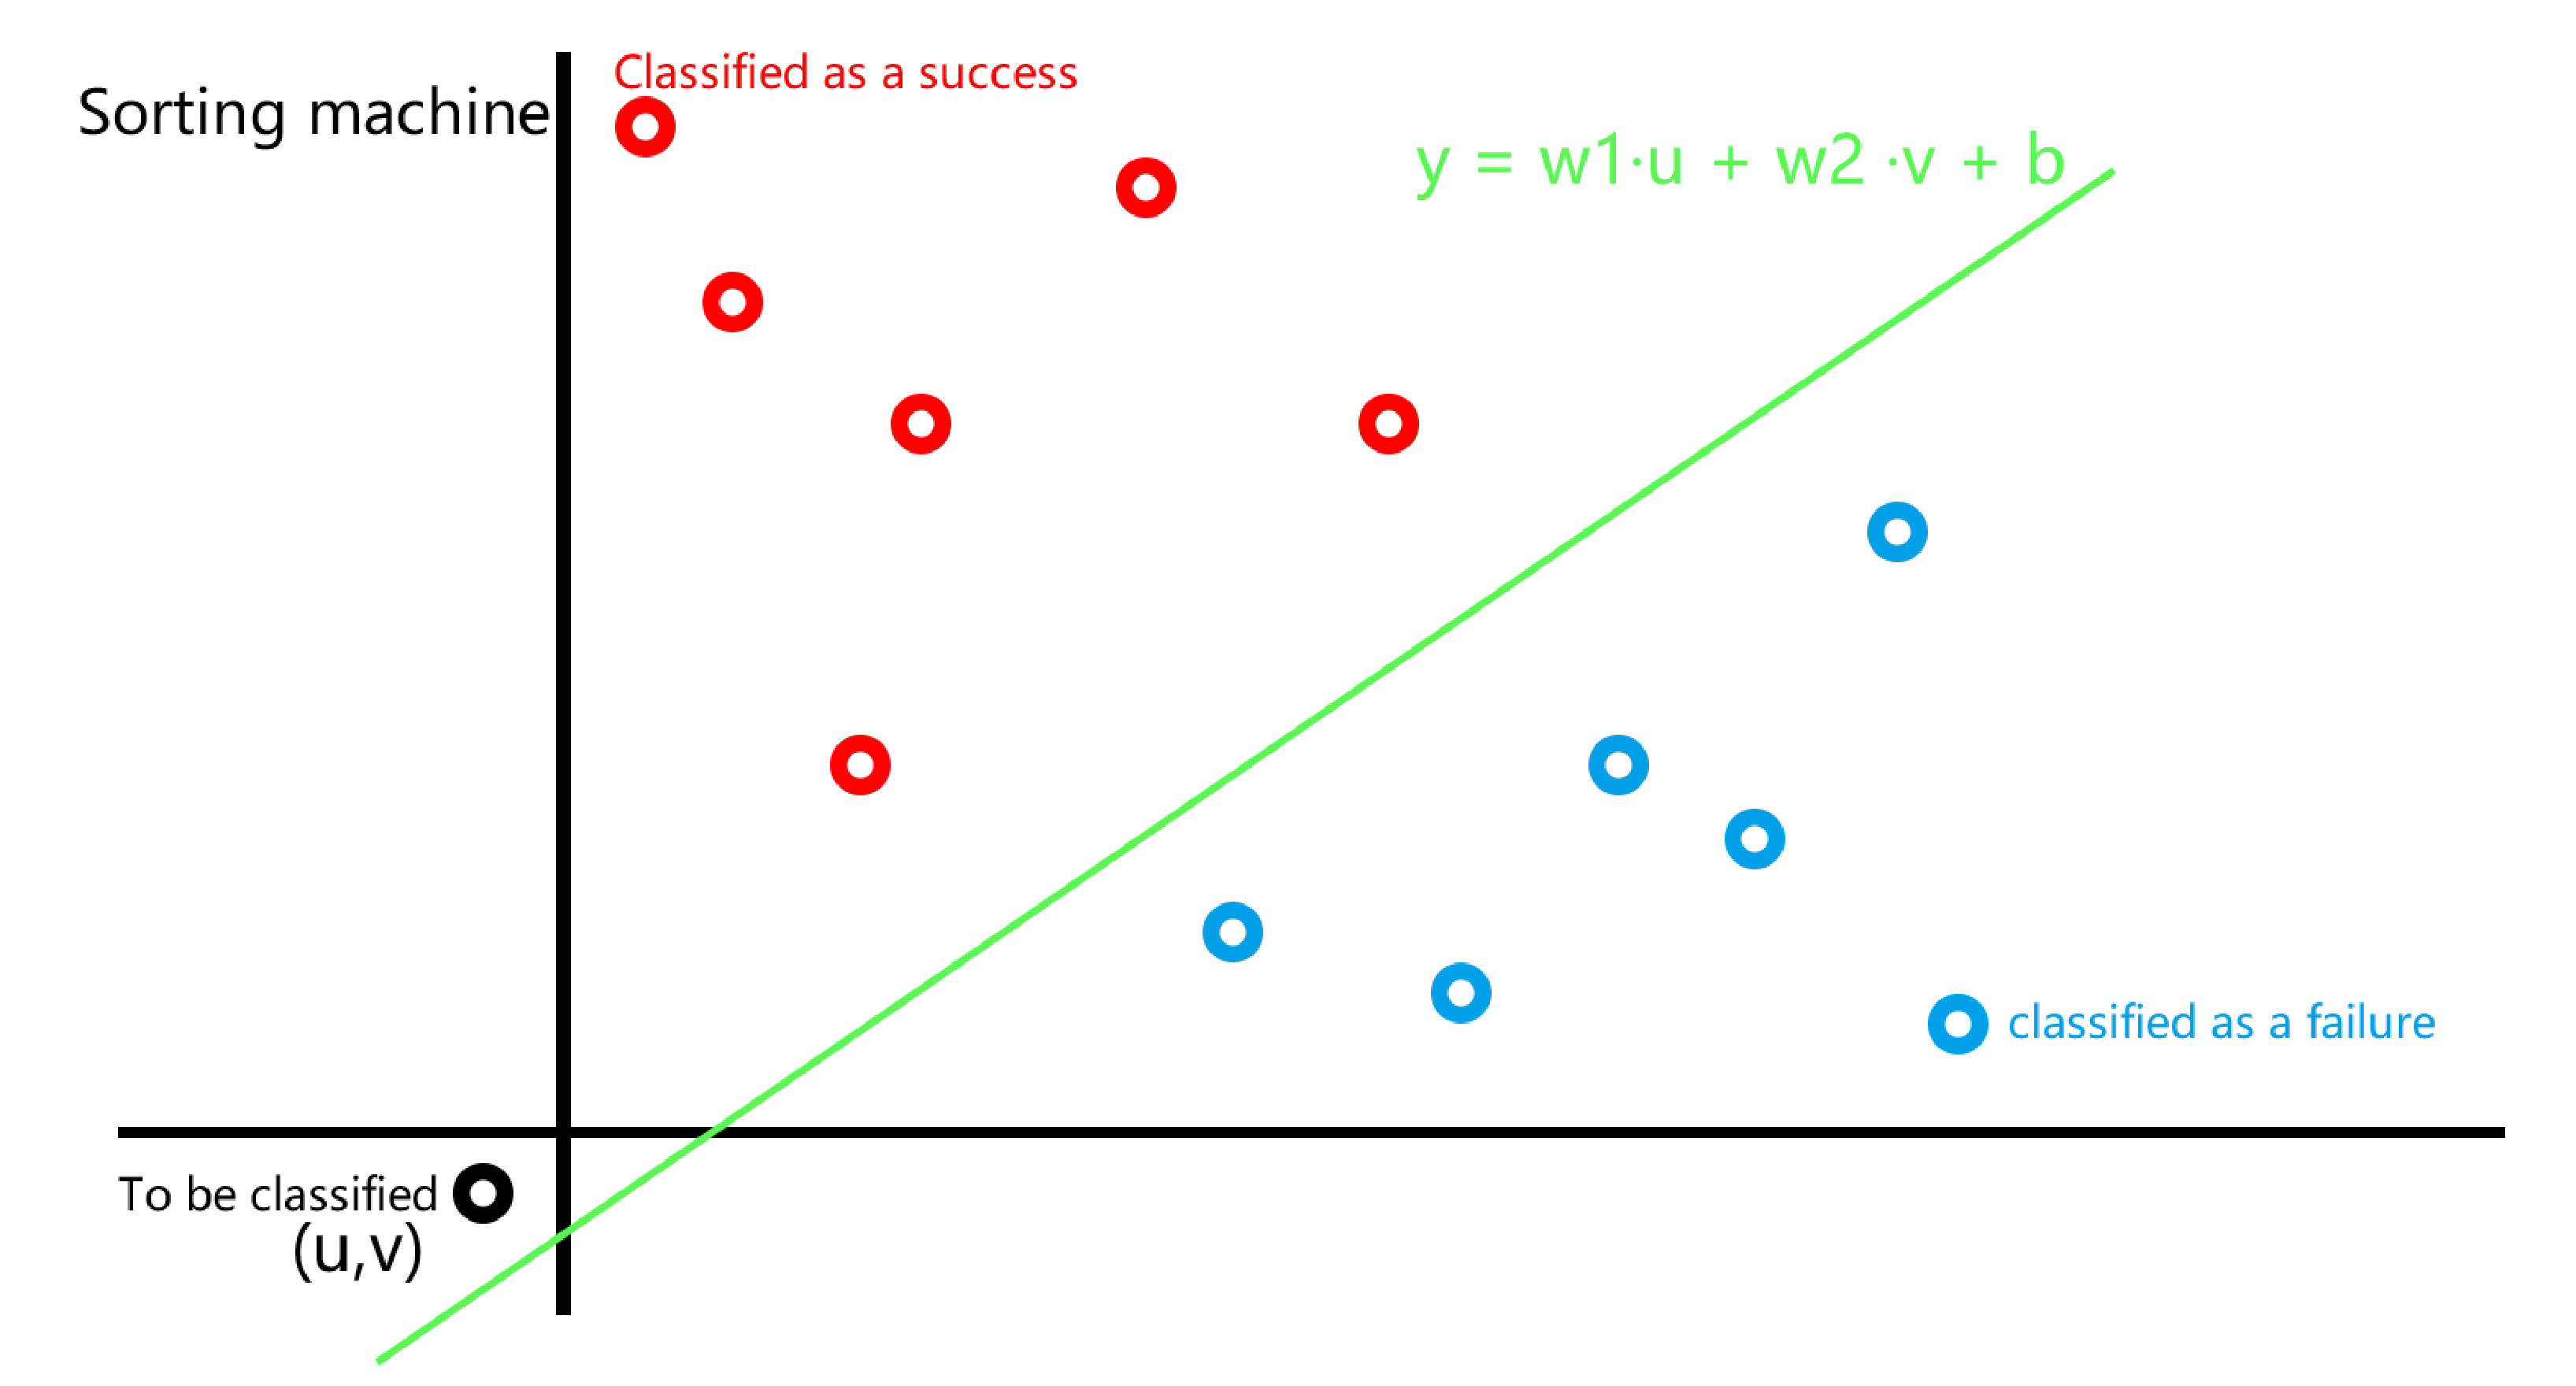
\includegraphics[width=1\textwidth]{Sortingmachine.eps}
 	\caption{Classification vector machine schematic}
\end{figure}

%%%%%%%%%
\textbf{\section{Model Simulation and Analysis}}
%%  5-1
\textbf{\subsection{Factor Analysis Results}}
\textbf{\subsubsection{SPSS Factor Analysis Processing Results}}

\begin{table}[htbp] %%%%表格
\caption{KMO and Bartlett inspection }  
	\centering
	\begin{tabular}{p{3.5cm}<{\centering}p{3.5cm}<{\centering} p{3.5cm}<{\centering}} 
		\toprule[1.5pt]
	product  &$ KMO $ & $Sig.$\\ 
		\midrule 
	$hair dryer $&0.740		& $0.000$  \\
	$microwave$	&0.753	&  $0.000$  \\
	$pacifier $	&0.754	& $ 0.000$  \\
		\bottomrule[1.5pt] 
	\end{tabular} 
\end{table}

Analysis: As can be seen from the above, their KMO values are all greater than 0.7, and their Sig. Values are 0.000, all of which are less than 0.05. In summary, it is suitable for factor analysis.


%%%碎石图片

\begin{figure}[h]
  	\centering
	\includegraphics[width=1\textwidth]{screetest.eps}
 	\caption{scree test of three products}
\end{figure}

Analysis:From the gravel charts corresponding to the three products, it can be seen that they all become flat after 2 factors, therefore for the three products, we extract two factors.


%%%组件图
 \begin{figure}[h]
  	\centering
	\includegraphics[width=1\textwidth]{zujiantu.eps}
 	\caption{component diagram in space after rotation of three products}
\end{figure}
Analysis:From the figure we can intuitively conclude that factor 1 consits of star rating constitutes, factor 2 consists of review title and review body.

%%解释方差
\begin{table}[htbp] %%%%表格
\caption{Weights of three products}  
	\centering
	\begin{tabular}{p{3.5cm}<{\centering}p{3.5cm}<{\centering} p{3.5cm}<{\centering}} 
		\toprule[1.5pt]
	product  &$ \omega_1 $ & $ \omega_2 $\\ 
		\midrule 
	hair dryer &55.11\%  	& $44.89\%$  \\
	microwave	&56.75\%	&  $43.25\%$  \\
	pacifier 	&55.22\%  	& $ 44.78\%$  \\
		\bottomrule[1.5pt] 
	\end{tabular} 
\end{table}



\textbf{\subsubsection{Ultimate Result}}

From the analysis above, the ultimate evaluation score calculation formula can be derive from the star rating, reviews scores and the weights obtained from the solution.
\begin{equation}
	fin score   =  \omega_1\times ST+\omega_2\times RV
\end{equation}

%%% 三张最终分数曲线图
 \begin{figure}[h]
  	\centering
	\includegraphics[width=1\textwidth]{excel_tu.eps}
 	\caption{Final score of three products}
\end{figure}

%%%5-2
\textbf{\subsection{SPSS Time Series Results}}
\textbf{\subsubsection{Model Fitting Results}}
%%解释方差
\begin{table}[htbp] %%%%表格
\caption{Weights of three products}  
	\centering
	\begin{tabular}{p{3.5cm}<{\centering}p{3.5cm}<{\centering}p{3.5cm}<{\centering} p{3.5cm}<{\centering}} 
		\toprule[1.5pt]
	product  &$ R^2 $ & $Sig. $  &  Outliers\\ 
		\midrule 
	hair dryer &0.680 & 0.173   & 0 \\
	microwave	&0.844&  $0.697$ &0 \\
	pacifier 	&0.682  	& $ 0.722$ &0 \\
		\bottomrule[1.5pt] 
	\end{tabular} 
\end{table}

Analysis: All the stable $R^2$ values above are greater than 0, showing that the model's fitting effect works well. And all the significance is greater than 0.05 and the outliers are zero, which also reflects that the model fits well.
\textbf{\subsubsection{Model Prediction Results}}

%%% 评论数量曲线预测
 \begin{figure}[h]
  	\centering
	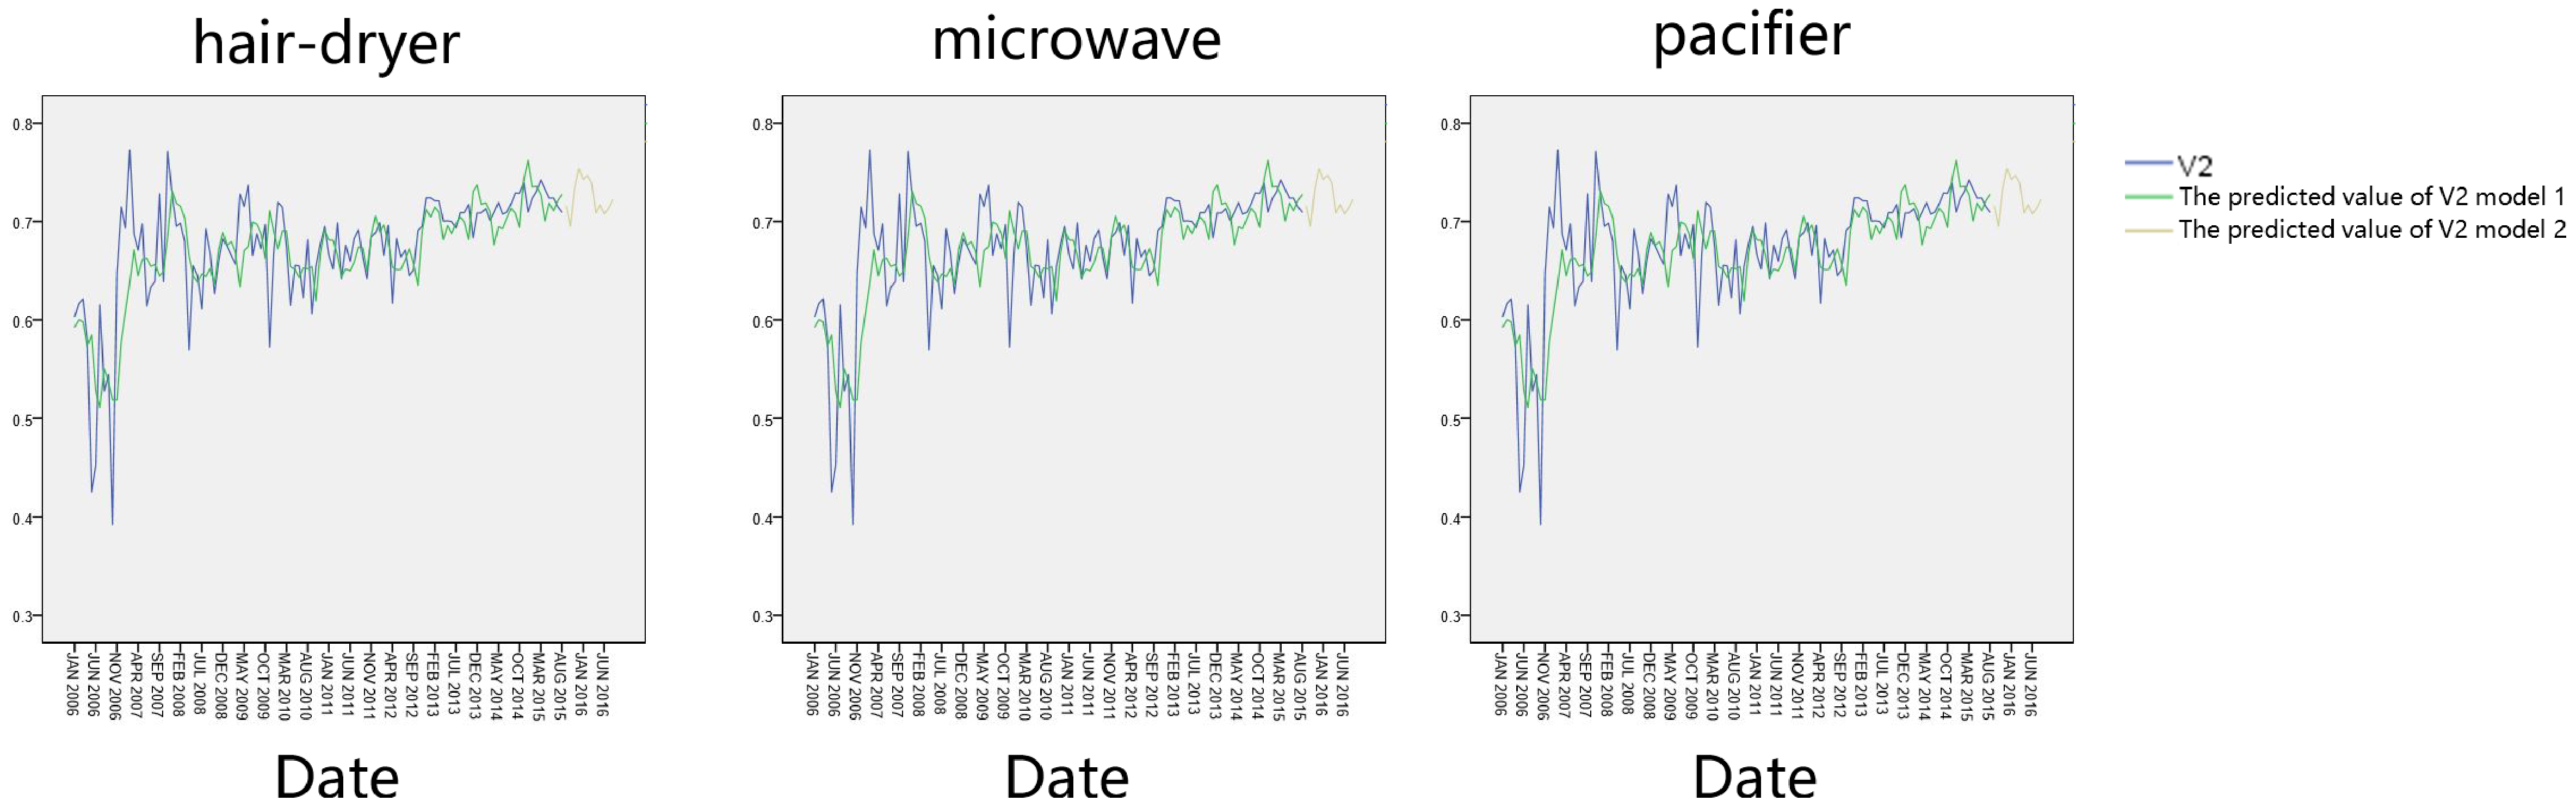
\includegraphics[width=1\textwidth]{B5.eps}
  	\caption{reviews amount}
\end{figure}
Analysis: Combined with the forecast chart, it can be intuitively seen that the number of monthly reviews of the three products is increasing over time, so the reputation of the three products can be considered to be rising.




%%% 平均分数曲线预测
 \begin{figure}[h]
  	\centering
	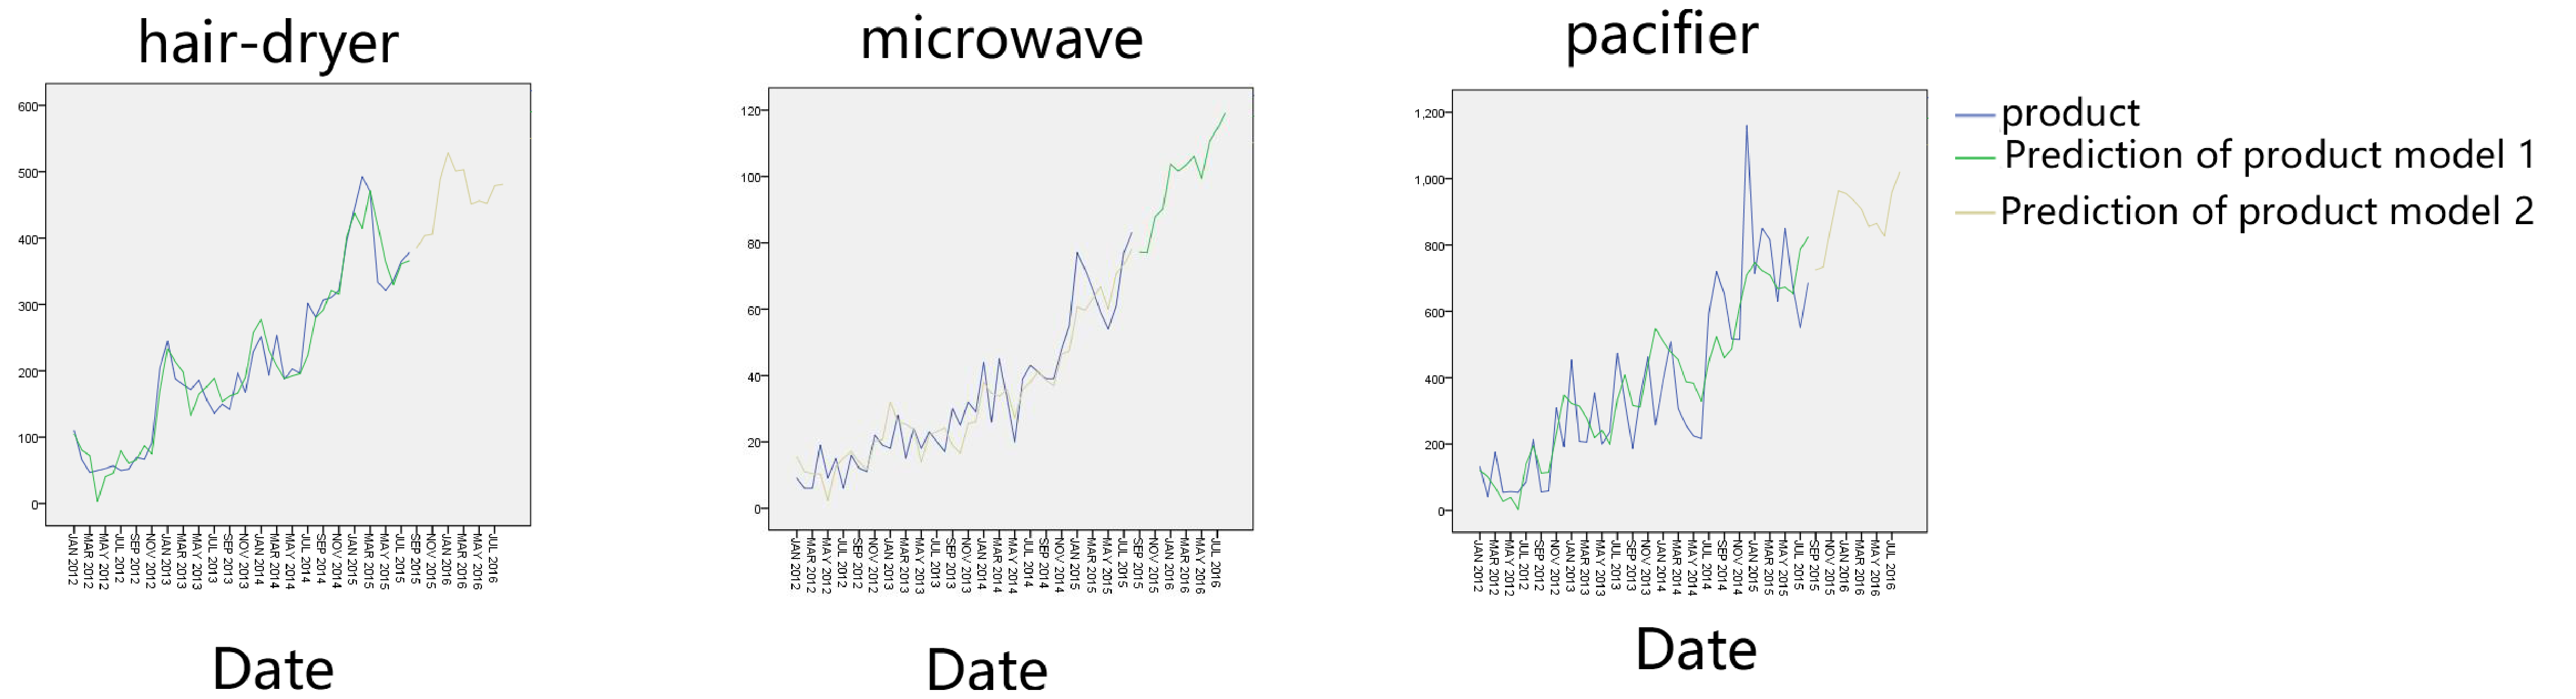
\includegraphics[width=1\textwidth]{B6.eps}
  	\caption{average score}
\end{figure}
Analysis: Combined with the forecast chart, we can know that the reputation of pacifier is decreasing, and the reputation of the other two groups of products are increasing.

Summary:Due to the more uncontrollable factors of the amount of reviews comparing with the average score, we think the average score is more representative of the reputation of the product. In summary, we firmly believe that the reputation of hair dryer and microwave is increasing, and the reputation of pacifier is decreasing.

%%%5-3
\textbf{\subsection{Analysis of Factors Affecting the Number of Reviews}}

People are always affected by the evaluation of others in life. Do high or low ratings from others lead to excessive reviews when shopping on Amazon? Or is the evaluation of those more appealing people (such as vine users) will make people more desire to write reviews? In order to find out the influence of these factors, we conducted the following investigation.

\paragraph{Analysis of the impact of high score and low score evaluation on the number of reviews}
We use the fitting method to find the impact of high and low evaluation on the number of reviews. The specific operation is to fit the time series from one star to five stars to the actual sequence of the total number of comments. Use i star (i = 1,2,3,4,5) as the independent variable x, the total number of comments as the dependent variable y, and fit with a linear function. Finally, we use the fitted function expression y = ax + b to display the degree of correlation. When a is larger, that is, the slope is larger, their correlation is higher. Because changes in the independent variable can cause changes in the dependent variable, which can cause more comments.
%%%%表格
%%%%表格
\begin{table}[htbp] %%%%表格
\caption{Weights of three products}  
	\centering
	\begin{tabular}{p{2.cm}<{\centering}p{2.cm}<{\centering}p{2.cm}<{\centering} p{2.cm}<{\centering}p{2.cm}<{\centering}p{2.cm}<{\centering}} 
		\toprule[1.5pt]
	product  &$ one star$ & twostar  &  three star&four star&five star\\ 
		\midrule 
	hair dryer &12.2368&17.6318&11.0311&5.7278&1.5943\\
	microwave	&4.0588&11.1924&8.5597&4.2058&2.1073\\
	pacifier 	&15.6569&20.3884&13.0396&7.2106&1.4651\\
		\bottomrule[1.5pt] 
	\end{tabular} 
\end{table}
%%%%%%
Analysis: From the data above, we can see that one or two stars will cause more reviews, and four or five stars will not have a large impact on the total number of reviews. So we consider that bad reviews will attract more reviews, while positive reviews won't.


\paragraph{Analysis of the influence of celebrity user reviews on the number of reviews}
Star effects often exist in our lives. This phenomenon manifests as vine users when shopping in Amazon. They are a kind of members who specialize in buying and making comments on products, and their evaluations of products often have more reference value. Below we discuss whether the evaluations of other customers will be affected after vine users giving evaluations.


Procedures are as follow, First of all, we will make a difference between the number of comments in this month and the number of comments in the previous month. Subtract last month's comments amount from this month's. It is positive if it increase, while is negative if it decrease. Then count the number of vine user reviews each month and divide them into two groups: positive (3 to 5 stars) and negative (1 to 2 stars). Calculate the change in their number of reviews next month to see if vine user reviews have an impact.


%%%%%%TUTU
%%% 饼状图
 \begin{figure}[h]
  	\centering
	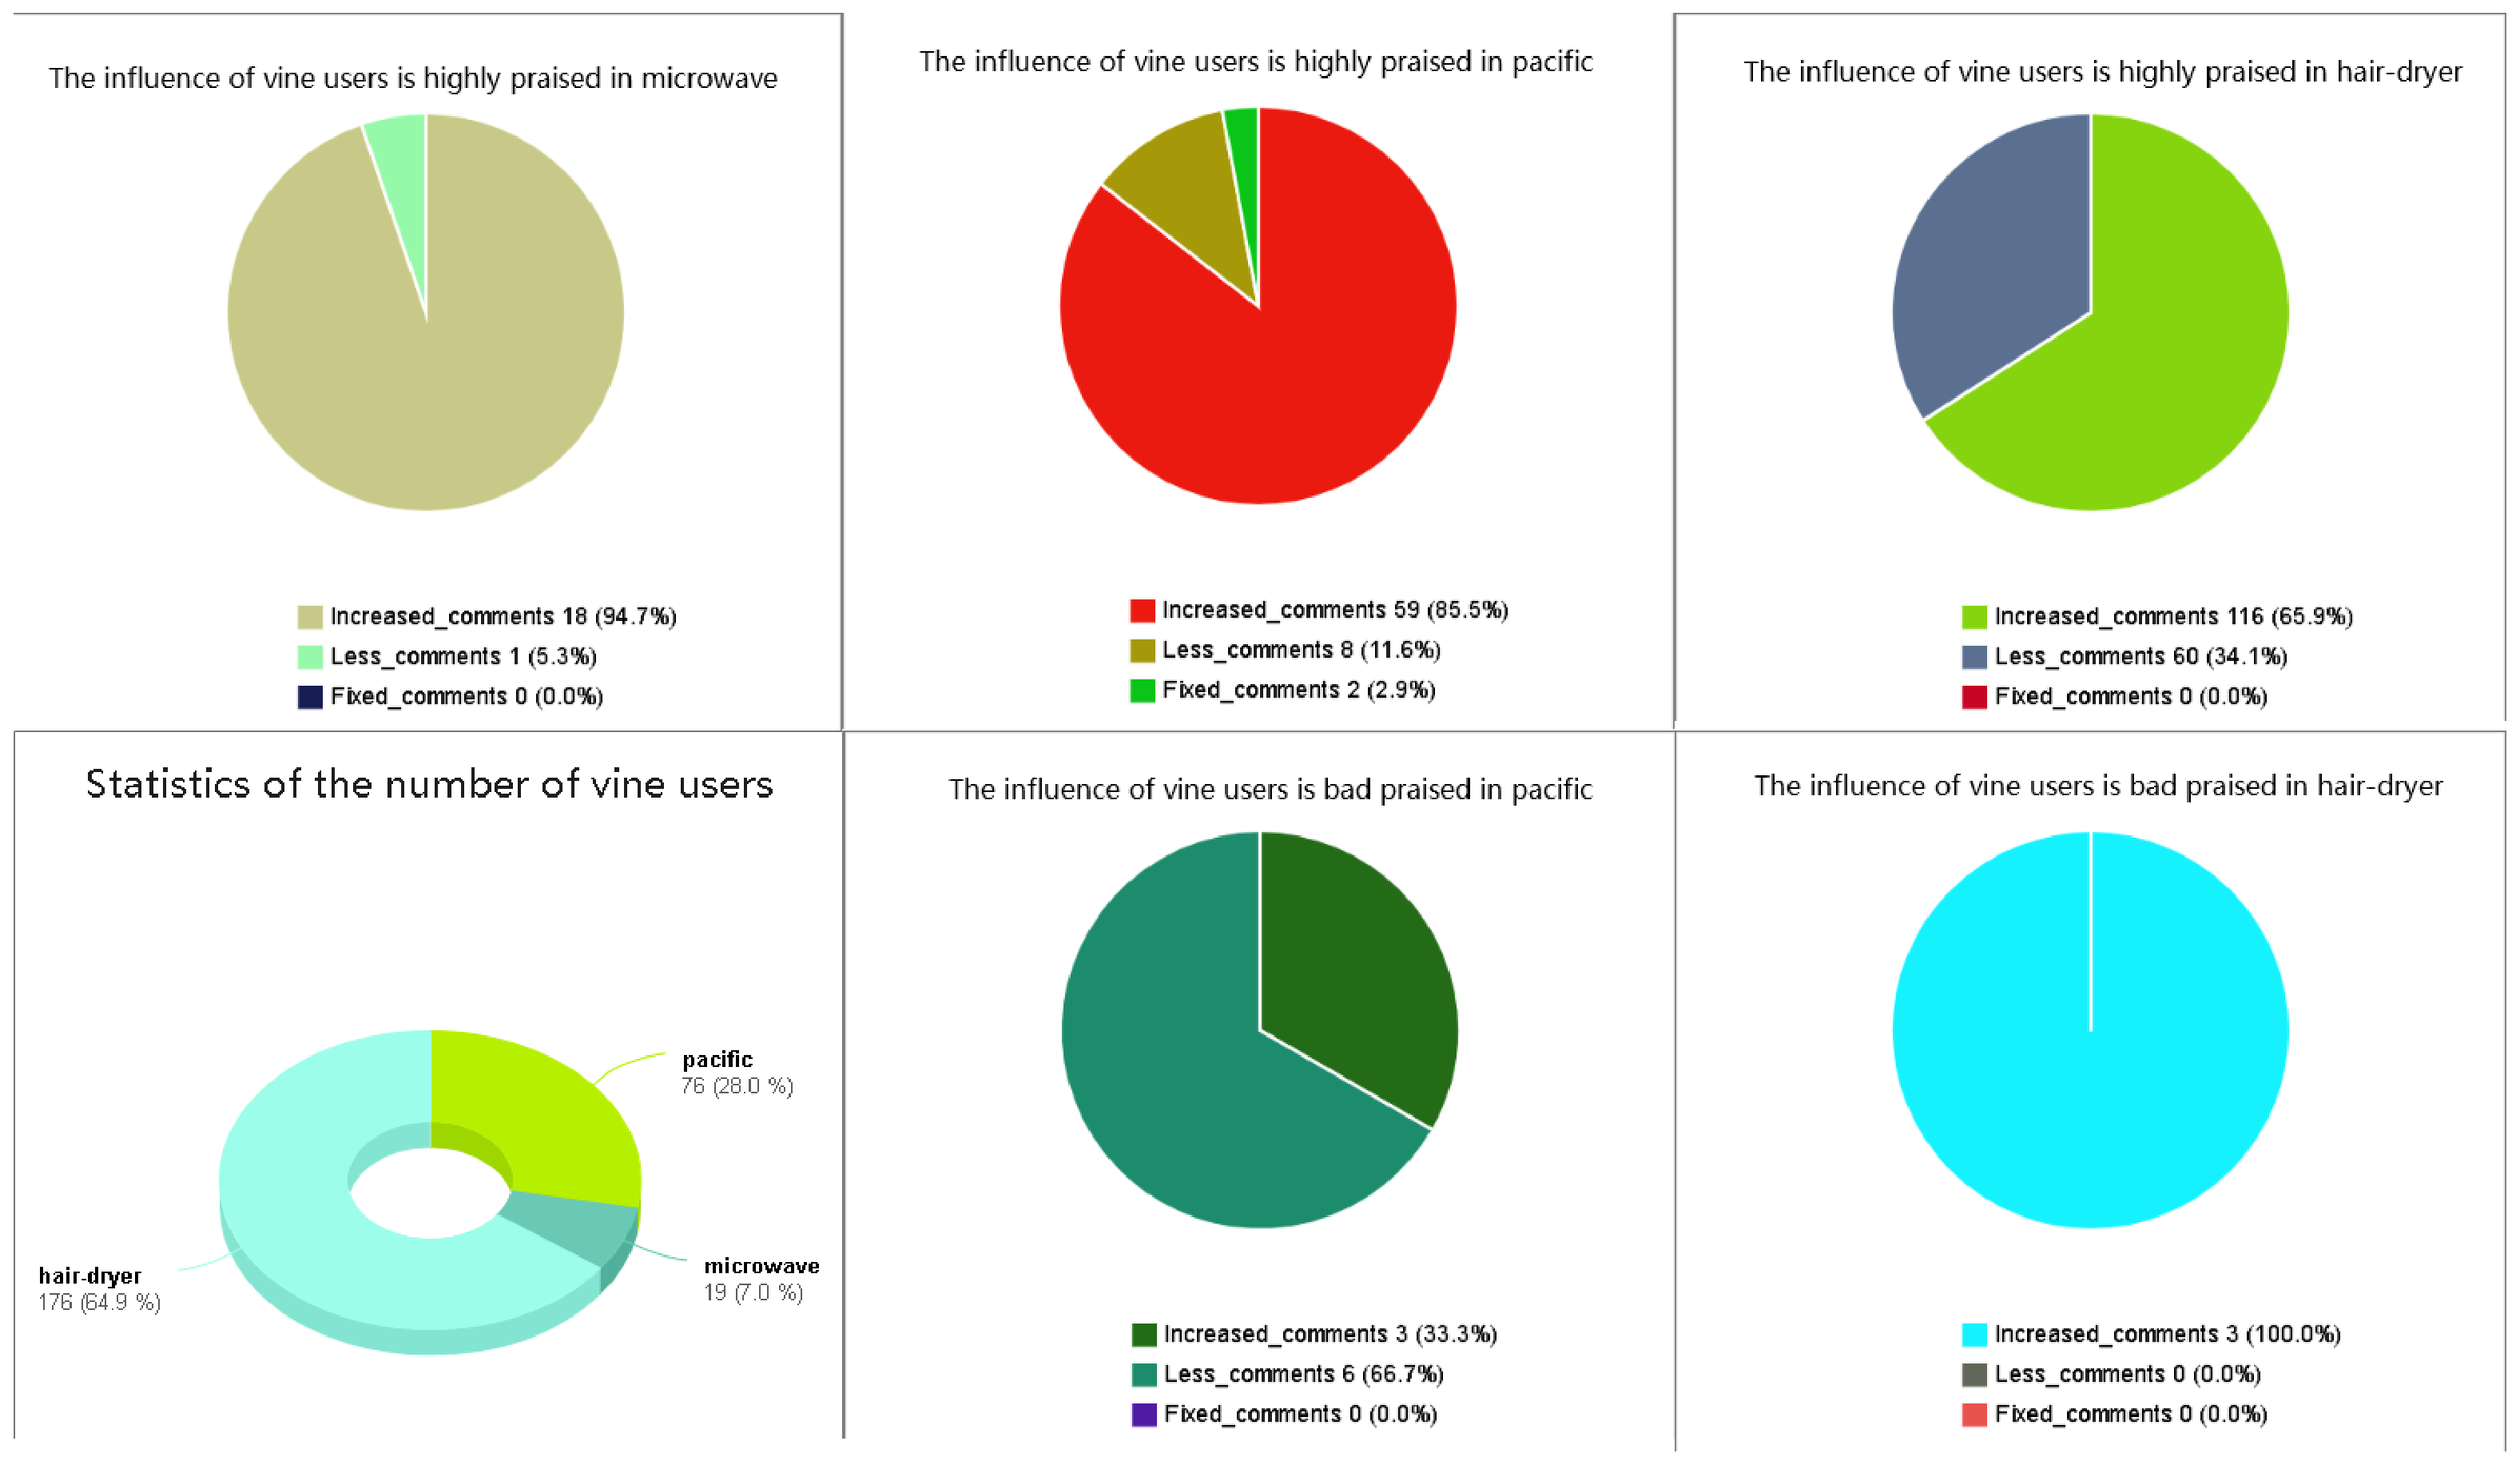
\includegraphics[width=1\textwidth]{huanzhuangtu.eps}
  	\caption{Impact of vine users on the number of reviews}
\end{figure}
Analysis: From the results above we can indicate that the comments of vine users may not cause more comments if they are negative, but if they are positive, it will have a significant effect on stimulating the increase in the number of comments.

%%%%%%%5-4
\textbf{\subsection{Correlation Analysis}}
Correlation analysis refers to the analysis of two or more variable elements with correlation to measure the closeness of the two variable factors.
In the previous calculation, we have rated the review based on its objective degree and negative direction, and calculated the weight of the review title and review body. The total review score can be derived from the combination of the review title and review body.
Next we will discuss the correlation between the star rating score and the review score for a product. SPSS is employed directly to perform correlation analysis. Pearson parameter is introduced here to perform analysis, which is used to measure whether datasets are excuted on the same perspective and measure linear relationship between distance variables. Here are the analysis results.

\begin{table}[htbp] %%%%表格
\caption{Correlation analysison on hair dryer datasets}  
	\centering
	\begin{tabular}{p{3.5cm}<{\centering}p{3.5cm}<{\centering} p{3.5cm}<{\centering}} 
		\toprule[1.5pt]
	      &$ star rating$ & $review $\\ 
		\midrule 
	star rating &1	& $0.923$  \\
	review	&0.923	&  $1 $  \\
	
		\bottomrule[1.5pt] 
	\end{tabular} 
\end{table}


\begin{table}[htbp] %%%%表格
\caption{Correlation analysison on microwave datasets}  
	\centering
	\begin{tabular}{p{3.5cm}<{\centering}p{3.5cm}<{\centering} p{3.5cm}<{\centering}} 
		\toprule[1.5pt]
	      &$ star rating$ & $review $\\ 
		\midrule 
	star rating &1	& $0.903$  \\
	review	&0.903	&  $1 $  \\
	
		\bottomrule[1.5pt] 
	\end{tabular} 
\end{table}

\begin{table}[htbp] %%%%表格
\caption{Correlation analysison pacifier datasets}  
	\centering
	\begin{tabular}{p{3.5cm}<{\centering}p{3.5cm}<{\centering} p{3.5cm}<{\centering}} 
		\toprule[1.5pt]
	      &$ star rating$ & $review $\\ 
		\midrule 
	star rating &1	& $0.766$  \\
	review	&0.766	&  $1 $  \\
	
		\bottomrule[1.5pt] 
	\end{tabular} 
\end{table}

It is found that there is a certain correlation between star rating and review based on the correlation between the star rating score and the review score of each product. For both microwave ovens and hair dryers,
The star rating score and the review score are even more strongerly relevant, which indicates that for most people, they are more willing to make objective and positive comments when they leave a higher star rating.

%%%%%%%%优缺点分析
\textbf{\section{Strengths and Weaknesses}}
Based on the modeling process, we make some comments on our model as listed below.
\textbf{\subsection{Strengths}}
\begin{itemize}
	\item After getting the data about the star rating, review title, and review body, we normalized the data, and then cleverly used SPSS's factor analysis to deal with the weight of each factor on the total score.
	\item Regarding the time-based analysis and research of data, although the time series problem is more complicated, SPSS solves the complicated part of the time series, so the part of the time series model is simplified.
	\item Using a classification vector machine and a sufficiently large data set, an optimal function for predicting potential success or failure can be obtained.
\end{itemize}
\textbf{\subsection{Weaknesses}}
\begin{itemize}
	\item The classification vector machine is used to deal with problems that indicate success or failure. After all, the solved data set does not reach the million level, so there will be overfitting problems to a certain extent.
	\item Regarding the processing of whether different star ratings will cause more comments, our model does not consider the time delay, that is, does not select a sufficient period of time to observe whether the number of reviews has increased.
\end{itemize}

\textbf{\section{Sensitivity Analysis}}
In the time series, the time interval T is set to one month. Next, we will change this value and observe the effect of the change with T on the model. Hair dryer datasets is employeed here as a analysis sample.
First take T as a benchmark. The sensitivity of our time series model could be obtained by analyzing the change in the fitting degree to the sales volume caused by the transformation of time interval T. As for the criterion of the degree of fit, the calculation of correlation is used to express.
Next is the correlation between sales and star ratings.

\begin {figure}[h]
	\centering % 居中显示
	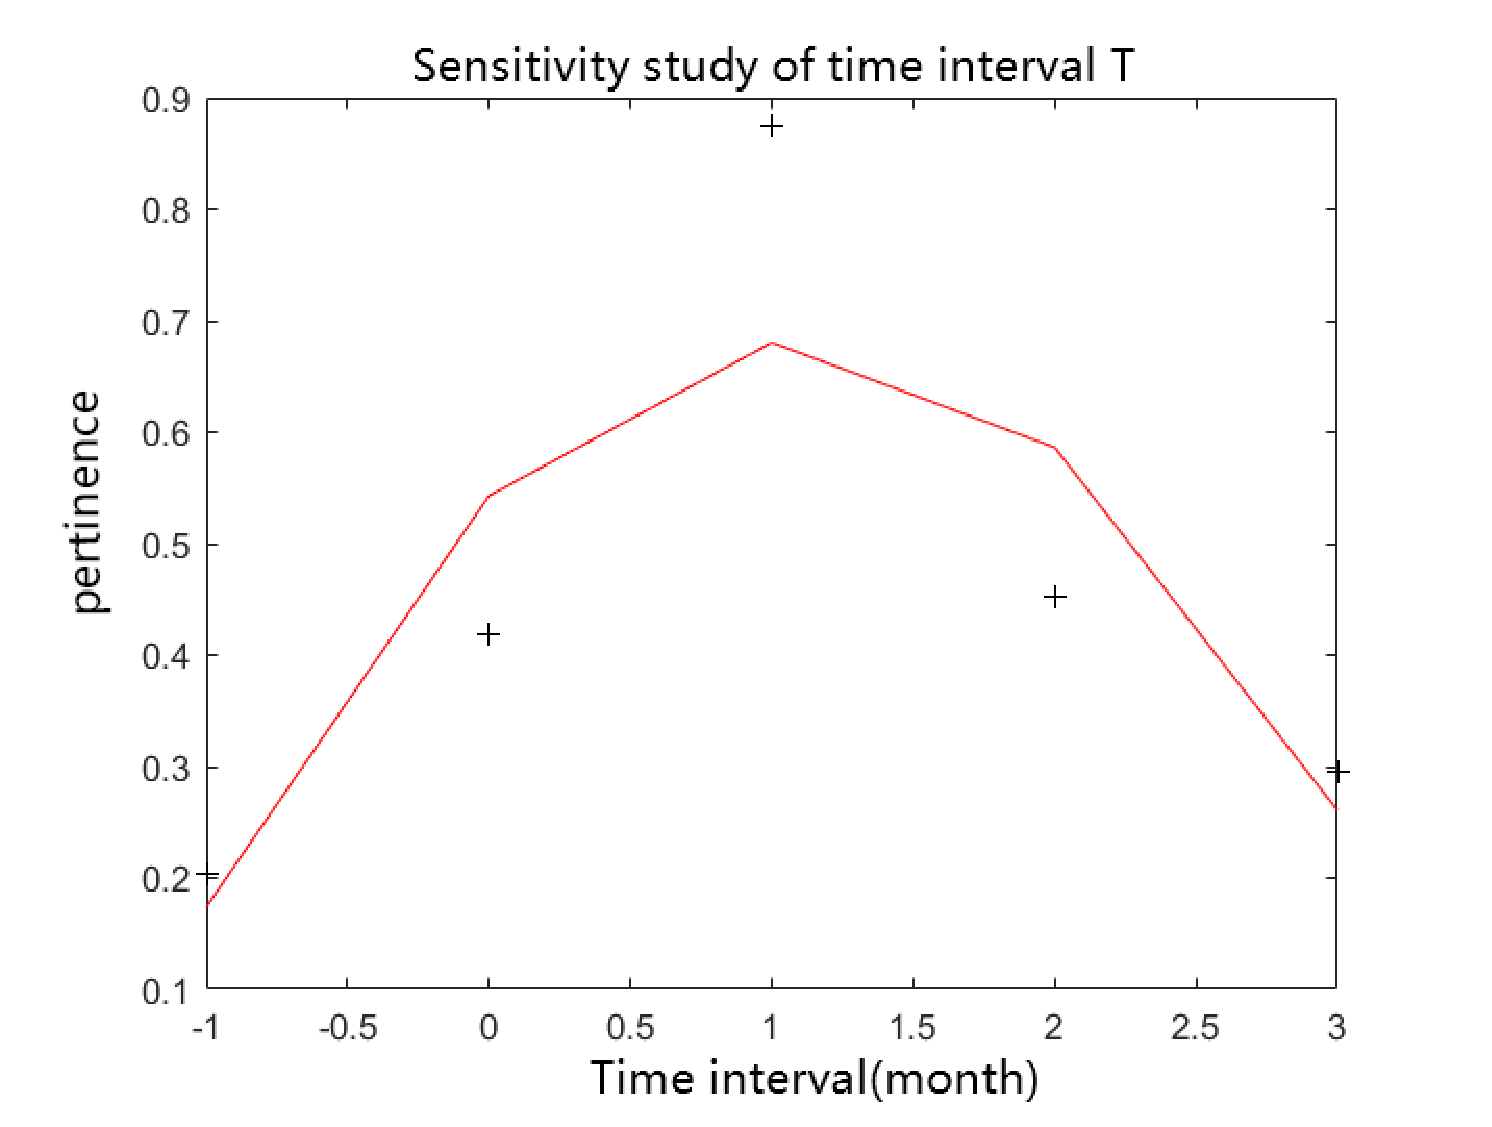
\includegraphics[width=14cm,height=11cm]{lmd.eps}
	\caption{shows that our time model is sensitive about the time interval T, and the best results are obtained when T is taken for one month.} % 标题
	\label{sensi}
\end {figure}




% 因为不输出此部分到目录 \addcontentsline{}{}{}是添加此标题到目录 
\newpage
\textbf{\section*{References}\addcontentsline{toc}{section}{References}}

\begin{thebibliography}{99}  
\bibitem{ref1}Mudambi S M.SchuffD., What Makes A Helpful Online Review? A Study of Customer Reviews on Amazon.com[J], MIS Quarterly, 2010,34(1):185-200.  
\bibitem{ref2}Kohli R,Devargj S,And Mahmood M A.Understanding Determiants of Online Consumer Satisfaction: A Decision Process Perspective[J],Journal of Management Information System,2004,21(1):115-135.  
\bibitem{ref3}Dan Zhang, Licheng Jiao, Xue Bai, Shuang Wang, Biao Hou,A robust semi-supervised SVM via ensemble learning[J],Applied Soft Computing,2018:632-643.  
\bibitem{ref4}Abhilasha Singh Rathor, Amit Agarwal, Preeti Dimri.Comparative Study of Machine Learning Approaches for Amazon Reviews[J],Procedia Computer Science,2018,1552-1561.  
\bibitem{ref5}Sung Guen Kim, Juyoung Kang.Analyzing the discriminative attributes of products using text mining focused on cosmetic reviews[J],Information Processing \& Management,2018,938-957.  
\bibitem{ref6}Mathwick C,Rigdon E.Play Flow and The Online Search Experience[J],Journal of Consumer Research,2004,31(2):324-332.
\bibitem{ref7}Ping Jiang, Hufang Yang, Jiani Heng.A hybrid forecasting system based on fuzzy time series and multi-objective optimization for wind speed forecasting[J],Applied Energy,2019,786-801.  
\end{thebibliography}
\end{document}